\section{Optimization-based open-loop control}\label{sec:flip}
The flip maneuver is a 360 degree rotation around one of the horizontal axes of the quadcopter body frame. In the literature there are several different approaches to perform the maneuver, for example based on apprenticeship learning \cite{abbeel2010}, energy-based control \cite{energy-quaternion}, or Lyapunov method \cite{lyapunov-flip}. We decided to first apply an  open-loop control method based on the optimization of a parametrized motion primitive sequence \cite{LSICRA2010}.

In this section, firstly the 2D equations of motion of the quadrotor are derived that is suitable for the applied control method. Afterwards, the parametrized primitive is described which consists of the sections of the maneuver, both beginning and ending in hover mode. Finally, the optimization problem of the primitive parameters is presented, and two different methods for the solution. 
%With the optimised parameter set, simulation results will be demonstrated. Finally, the implementation of the flip controller on the Crazyflie quadrotor, and experimental results will be discussed.

\subsection{2D Quadrotor model}

In this section, a two dimensional dynamic model of the quadcopter is used as the desired trajectory of the flip motion is within the $x-z$ plane of the body frame. The model consists of the thrust and moment of the four rotors, and the gravitational field. Other dynamics, such as the vehicle yaw are stabilized separately and are now ignored. Unlike the maneuver described in \cite{LSICRA2010}, we use $\times$ configuration as two rotors can produce a larger torque for the flip than one. From the Newtonian equations of motion using the direction conventions displayed in Figure \ref{fig:flipframe} and Euler angle representation:
\begin{align}
m\ddot{x}&=-(T_1 + T_2 + T_3 + T_4)\sin\theta,\\
m\ddot{z}&=-(T_1 + T_2 +T_3 + T_4) \cos\theta+mg,\\
J_{yy}\ddot{\theta} &= l(T_1+T_4-T_2-T_3),\label{eq:opinp1}
\end{align}

\begin{figure}[b]
\centering
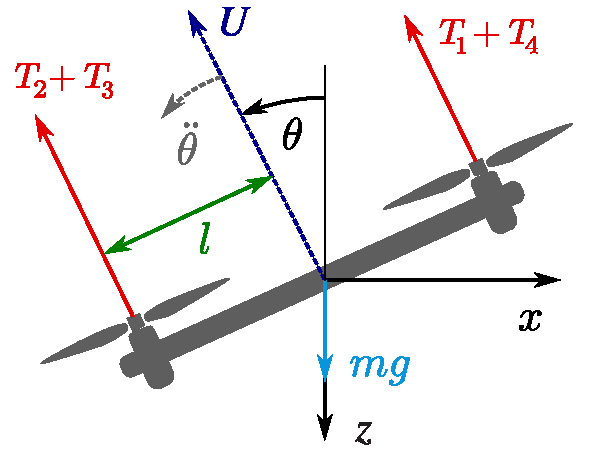
\includegraphics[width=.35\textwidth]{Fig/flip_frame_2.pdf}
\caption{The vehicle frame, the orientation and forces acting on the quadcopter in two dimensions.}\label{fig:flipframe}
\end{figure}

where $\theta$ is the pitch angle, $g$ is the gravitational acceleration, $m$ is the mass of the drone, $l$ is the distance of a propeller from the center of mass of the vehicle, $J_{yy}$ is the moment of inertia about the axis of the flip (out-of-plane principal axis), and $T_i,$ $i=1,2,3,4$ are the thrusts of each rotor. The collective acceleration $U$ is the sum of all rotor thrusts divided by the mass of the drone,
\begin{equation}
U = \frac{T_1 + T_2 + T_3 + T_4}{m}.\label{eq:opinp2}
\end{equation}
As the small DC motors of the Crazyflie 2.1 have very small time constants the actuator dynamics are omitted.% The physical parameters of the model are contained in Table x, mostly determined from \cite{Forster}.


\subsection{Parametrized primitive of the maneuver}\label{sec:sections}
The goal of the maneuver is to perform a flip, therefore the states at the start and end should be the same, except for the pitch angle which is offset by $2\pi$. From these considerations, the initial and final state conditions for the maneuver can be formulated as:
\begin{subequations}
\begin{align}
x_0 = x_f &= 0,\\
z_0 = z_f &= 0,\\
\dot{x}_0 = \dot{x}_f = \dot{z}_0 = \dot{z}_f &= 0,\\
\theta_f = \theta_0 + 2\pi &= 0.
\end{align}
\end{subequations}
We use a simple control approach without explicit optimization for execution time. Research has shown that for different types of dynamic systems, bang-bang control strategies provide near-optimal results, with small complexity \cite{KALMARNAGY2004,tdk2019}. We use such control actions within a restricted control envelope, denoted as a range of accelerations $[\underline{\beta},\overline{\beta}]$, in order to take into consideration modelling uncertainties and reserve some resources for the on-board stabilizing controller. This restriction can be mathematically formulated for the rotating rotor thrusts as
\begin{align}
T_\mathrm{min} \leq \frac{m\underline{\beta}}{4}\leq F_{i} \leq\frac{m\overline{\beta}}{4} \leq T_\mathrm{max}.
\end{align}
The control strategy of the maneuver consists of five sections, all of which has two constant inputs, the desired collective acceleration $U_\mathrm{des}$, and desired angular acceleration $\ddot{\theta}_\mathrm{des}$. These five steps are illustrated in Figure \ref{fig:sections}, and defined as follows.
\renewcommand{\baselinestretch}{0.85}\normalsize 
\begin{enumerate}
\item \textbf{Accelerate:} Gain elevation and kinetic energy with nearly maximum collective acceleration, while rotating slowly to the negative direction.
\item \textbf{Start Rotate:} Increase angular velocity with torque, i.e. maximal differential thrust.
\item \textbf{Coast:} With low and uniform thrusts hold the angular velocity, wait for the drone to rotate.
\item \textbf{Stop Rotate:} Use maximal differential thrust to decrease angular velocity and stop the rotation.
\item \textbf{Recover:} Prevent the drone from falling to the ground by applying nearly maximal collective thrust, and try to get back to hover mode.
\end{enumerate}
\renewcommand{\baselinestretch}{1.15}\normalsize

\begin{figure}
\centering
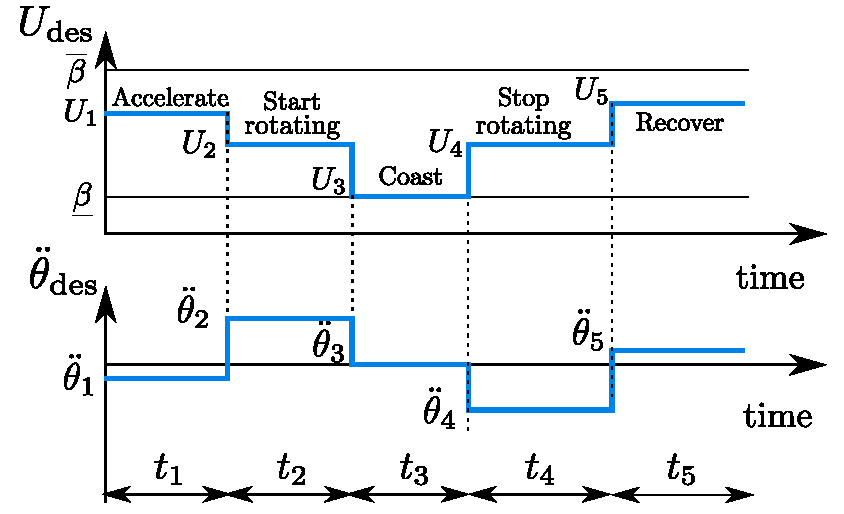
\includegraphics[scale=.7]{Fig/sections2.pdf}
\caption{Parametrized flip primitive with the five sections.}\label{fig:sections}
\end{figure}

Each section has three parameters, the collective acceleration $U_i$, duration $t_i$, and angular acceleration $\ddot{\theta}_i$. Since we use the properties of bang-bang control, $U_i$ and $\ddot{\theta}_i$ fully determine each other. Based on \cite{LSICRA2010}, we select 
\begin{align}
P=\begin{bmatrix}\label{eq:openparams}
U_1 & t_1 & t_3 & U_5& t_5
\end{bmatrix} ^\top
\end{align} as the parameters to optimize, and calculate the other ten quantities as detailed in the paper. The calculation of an initial guess is also discussed in \cite{LSICRA2010}, which we utilize in the implementation.

From the parameters, the control input vector can be calculated as
 \begin{align}\label{eq:openinp}
    \begin{bmatrix}
        F_i \\ \tau_i
    \end{bmatrix}=\begin{bmatrix}
        mU_i \\ 0 \\ J_{yy}\ddot{\theta}_i \\ 0
    \end{bmatrix},
\end{align}   
where $m$ is the mass of the quadcopter.

\subsection{Parameter optimization via numerical simulations}
The five parameters are tuned in order to minimize the norm of the final state error $E$, mathematically described as
\begin{subequations}\label{eq:optim}
\begin{align}
E &= \begin{bmatrix}
x_f & z_f & \dot{x}_f & \dot{z}_f & \theta_f
\end{bmatrix}^\top,\\
P^* &= \argmin_P \|E\|_2.
\end{align} 
\end{subequations}

In the original paper \cite{LSICRA2010}, the numerical optimization of the five parameters is based on iterative learning, using the approximate Jacobian matrix of the final state error w.r.t the parameter vector. However, the numerical gradient approximation has vast computational cost, because the whole maneuver needs to be simulated in every approximation step. Hence we have chosen Bayesian optimization which does not require any functional form and is suitable for global optimization of cost functions that are expensive to evaluate \cite{frazier2018tutorial, bayesopt2, brochu2010tutorial}.

The main concept of Bayesian optimization is to treat the unknown objective function as a random function in a parametric structure, fit the model parameters using Bayesian inference techniques, and maximize the output of the fitted surrogate model. The high-level steps of the optimization method are described in Algorithm \ref{alg:bayes}.
\begin{algorithm}
\caption{Basic pseudo-code for Bayesian optimization \cite{frazier2018tutorial}}
\label{alg:bayes}
\begin{algorithmic}[1]
	\State Place a Gaussian process prior on $f$
    \State Observe $f$ at $n_0$ initial points, set $n=n_0$
    \While {$n\leq N$}
    \State Update the posterior probability distribution on $f$ using all available data
    \State Let $x_n$ be a maximizer of the acquisition function over $x$, where the acquisition function is computed using the current posterior distribution
    \State Observe $y_n = f(x_n)$
    \State $n=n+1$
	\EndWhile
	\State Return a solution: either the point evaluated with the largest $f(x)$, or the point with the largest posterior mean
\end{algorithmic}
\end{algorithm}

There are multiple methods to define the parametric structure, the most common of which is using \textit{Gaussian processes} (GPs) \cite{GPMPC2019}. GP provides a flexible, nonlinear structure representing a single layer neural network, depends on relatively few parameters and its training is fast and efficient. Moreover, the covariance of GP gives a measure of the uncertainty of the approximation which is then used to systematically select the next evaluation point of the optimizer, and thus help the balance between exploration and exploitation.

By definition, a Gaussian process $\mathcal{GP}: \mathbb{R}^{d} \rightarrow \mathbb{R}$ is a mapping that assigns to every point $x \in \mathbb{R}^{d}$ a random variable $\mathcal{G} \mathcal{P}(x) \in \mathbb{R}$ such that for any finite set $x^{(1)} \ldots x^{(n)}$ the joint probability distribution of $\mathcal{G} \mathcal{P}\left(x^{(1)}\right), \ldots, \mathcal{G} \mathcal{P}\left(x^{(n)}\right)$ is Gaussian with mean $m$ and covariance $K$, expressed as
\begin{subequations}
\begin{align}
m &=\left[m\left(x^{(1)}\right), \ldots m\left(x^{(n)}\right)\right]^{\top} \\
[K]_{i j} &=\kappa\left(x_{i}, x_{j}\right),
\end{align}
\end{subequations}
where $[\cdot]_{i j}$ denotes the $(i, j)$-th entry of a matrix and $\kappa$ is a suitable kernel function. Both the mean and kernel depend on the \textit{hyperparameters} denoted by $\theta$, which are tuned during the optimization process. The goal is to learn the objective function $f:\mathbb{R}^d \rightarrow \mathbb{R}$ using a training set generated from the function evaluations $(x, f(x))$. An intuitive interpretation of the training is to find the GP that is most probable to have generated the training set, assuming that $f$ is a sample of the GP. 

The training starts with model selection, i.e. choosing a suitable mean and kernel function. By subtracting the mean of the data from all elements, constant zero mean is a common choice. The kernel is the core of the GP, it characterizes the function class in which we search the objective function. For smooth functions with approximately constant characteristic length the Squared Exponential kernel is a common and good choice, but there are also more complex kernel functions, e.g. the Matérn class.

Next step of the training is hyperparameter tuning, most commonly obtained by maximizing the \textit{marginal likelihood} of the training samples with respect to $\theta$. For proper scaling, often the logarithm of the likelihood is maximized, characterized by
\begin{align}
\log p(\overline{y} \mid {X}, {\theta}) &=\log \int_{-\infty}^{\infty} p(\overline{y} \mid f, {X}, {\theta}) p(f \mid {\theta}) \mathrm{d} f,
%\\ &=\underbrace{-\frac{1}{2} {y}^{\top}\left({K}+\sigma_{\varepsilon}^{2} \mathbf{I}\right)^{-1} \mathbf{y}}_{\text {data-fit term }}-\underbrace{\frac{1}{2} \log \left|\mathbf{K}+\sigma_{\varepsilon}^{2} \mathbf{I}\right|}_{\text {complexity term }}-\frac{n}{2} \log (2 \pi)
\end{align}
where $\mathcal{T} = {(x^{(i)},\overline y^{(i)})}_{i=1}^n$ is the training set, $X=[x^{(1)}\dots x^{(n)}]$, $\overline y = [\overline y^{(1)}\dots \overline y^{(n)}]^\top$ and $p({y} \mid {X}, {\theta})$ denotes the $n$ dimensional joint Gaussian distribution of $\mathcal{GP}(x^{(1)})\dots\mathcal{GP}(x^{(n)})$. Since the gradient of the expression is easy to evaluate, a gradient ascent algorithm can be applied to maximize the marginal likelihood.

The evaluation of a trained GP, i.e. the approximation of $f$ at a test point $x_*\in\mathbb{R}^d$ is calculated as follows. We take the $n+1$ dimensional joint distribution $$p([y^{(1)},\dots,y^{(n)},y ] \mid [X,x_*],\theta),$$ and calculate the one dimensional conditional distribution $$p(y\mid x_*,y^{(1)}=\overline y^{(1)}, \dots ,y^{(n)}=\overline y^{(n)},X,\theta ).$$ The mean of this distribution $m_*$ is the approximation for $f(x_*)$, and the variance $\sigma_*$ gives a measure of the uncertainty of the regression. The evaluation of a GP requires only elementary matrix operations, therefore it is computationally efficient.

With a trained GP model and rules for the evaluation, we need an acquisition function to determine the next test point. The goal of the acquisition function is to balance between exploration and exploitation while trying to find the global maximum. The trade-off between exploration and exploitation is usually provided by maximizing the sum of the mean and variance of the posterior distribution scaled by different (and time dependent) gains. Common acquisition functions are expected improvement, knowledge gradient, and entropy search.

%The function evaluations are treated as data, based on which the posterior distribution is formulated over the objective function, using Bayes' theorem. The posterior distribution is then used to evaluate the acquisition function, and determine the next query point. With the growing number of data points, the posterior distribution will be more certain about which parts of the parameter space are worth exploring and which are not. The most common acquisition function is upper confidence bound (UCB). For the oncoming function evaluation, it always chooses the point from the parameter space where the upper confidence bound of the posterior distribution is the highest. This way, it provides a balance between exploration and exploitation, because if it would stuck in a local maximum, the confidence interval will become narrow, so the algorithm will start exploring the points with high uncertainty. 

%In most cases, Gaussian Processes (GPs) are used to define the prior and posterior distributions over the objective function. Research has shown that GP models are efficient nonlinear function approximators, especially for smooth functions with radial basis function (RBF) or Matérn kernel \cite{RW2006}.

With the mathematical model of the quadcopter and a suitable optimization algorithm, it is possible to simulate the maneuver with different parameter sets, optimize the motion, and implement on the vehicle. For the implementation of the open-loop flip, a stabilizing flight controller is also required to balance the quadcopter at the beginning and after the end of the maneuver. Setpoint stabilization is a common task in quadcopter control, a classical LTI feedback controller is suitable designed for the linearized dynamics around hovering, for example PID or LQR. 

It is important to note that parameter uncertainties are the bottleneck of open-loop control strategies, it is essential to have an accurate simulation model which can be adapted to the real system in case the dynamic behaviour of the vehicle changes. In the next section, a nonlinear geometric control approach is proposed that is more robust to parameter uncertainties due to feedback, therefore does not require such complex and accurate modeling of the quadcopter dynamics.

%Although a simulation program is presented in \cite{LSICRA2010}, it is highly simplified, and created for an old Python version and a different quadrocopter. Hence we decided to use an OpenAI Gym environment based on PyBullet \cite{gym}, and implement the flip controller within this framework. As the package is originally developed for reinforcement learning with drones, it is suitable both for our current objective and future goals.